\documentclass[a4paper]{article}


\usepackage[utf8]{inputenc}
\usepackage[T1]{fontenc}
\usepackage{textcomp}
\usepackage{mathtools,amssymb,amsthm}
\usepackage[top=2.5cm,bottom=2.5cm,right=2.5cm,left=2.5cm]{geometry}
\usepackage[francais]{babel}
\usepackage{appendix}

%================image=================
\usepackage{graphicx}
\graphicspath{{figures/}}
\renewcommand{\listfigurename}{Table des figures}

%============header and foot============
\usepackage{fancyhdr}
\pagestyle{fancy}
\renewcommand\headrulewidth{1pt}
\fancyhead[L]{\bfseries Tests unitaires}
\fancyhead[R]{
\includegraphics[scale=0.05]{./img_rapport/prepisima.png}}
\fancyfoot[L]{CHASSAGNOL Rémi et CLIQUOT Théo}
\fancyfoot[R]{2020-2021}

% =================other================
\renewcommand{\texttt}[2][blue]{\textcolor{#1}{\ttfamily #2}}
\renewcommand{\contentsname}{Table des matières}
\usepackage{multicol}
\newcommand{\dollar}{\mbox{\textdollar}}
%=================code=================
\usepackage{verbatim}
\usepackage{listings}
\usepackage{color}
\usepackage[table]{xcolor}
\usepackage[most]{tcolorbox}
%==============code settings==========
\definecolor{my_gray}{rgb}{0.20,0.20,0.55}
\definecolor{darkWhite}{rgb}{0.97,0.97,0.97}
\definecolor{myred}{rgb}{1,0.22,0.22}
\definecolor{mypurple}{rgb}{0.74,0.36,0.97}
\lstset{
   literate=
  {á}{{\'a}}1 {é}{{\'e}}1 {í}{{\'i}}1 {ó}{{\'o}}1 {ú}{{\'u}}1
  {Á}{{\'A}}1 {É}{{\'E}}1 {Í}{{\'I}}1 {Ó}{{\'O}}1 {Ú}{{\'U}}1
  {à}{{\`a}}1 {è}{{\`e}}1 {ì}{{\`i}}1 {ò}{{\`o}}1 {ù}{{\`u}}1
  {À}{{\`A}}1 {È}{{\'E}}1 {Ì}{{\`I}}1 {Ò}{{\`O}}1 {Ù}{{\`U}}1
  {ä}{{\"a}}1 {ë}{{\"e}}1 {ï}{{\"i}}1 {ö}{{\"o}}1 {ü}{{\"u}}1
  {Ä}{{\"A}}1 {Ë}{{\"E}}1 {Ï}{{\"I}}1 {Ö}{{\"O}}1 {Ü}{{\"U}}1
  {â}{{\^a}}1 {ê}{{\^e}}1 {î}{{\^i}}1 {ô}{{\^o}}1 {û}{{\^u}}1
  {Â}{{\^A}}1 {Ê}{{\^E}}1 {Î}{{\^I}}1 {Ô}{{\^O}}1 {Û}{{\^U}}1
  {œ}{{\oe}}1 {Œ}{{\OE}}1 {æ}{{\ae}}1 {Æ}{{\AE}}1 {ß}{{\ss}}1
  {ű}{{\H{u}}}1 {Ű}{{\H{U}}}1 {ő}{{\H{o}}}1 {Ő}{{\H{O}}}1
  {ç}{{\c c}}1 {Ç}{{\c C}}1 {ø}{{\o}}1 {å}{{\r a}}1 {Å}{{\r A}}1
  {€}{{\EUR}}1 {£}{{\pounds}}1,
  mathescape,
  aboveskip=3mm,
  belowskip=-2mm,
  backgroundcolor=\color{darkWhite},
  basicstyle=\ttfamily\footnotesize,
  breakatwhitespace=false,
  breaklines=true,
  captionpos=b,
  commentstyle=\color{myred},
  deletekeywords={...},
  escapeinside={\%*}{*)},
  extendedchars=true,
  framexleftmargin=16pt,
  framextopmargin=3pt,
  framexbottommargin=6pt,
  frame=tb,
  keepspaces=true,
  keywordstyle=\color{mypurple},
  morekeywords={*,...},
  numbers=left,
  numbersep=10pt,
  numberstyle=\tiny\color{black},
  rulecolor=\color{black},
  showspaces=false,
  showstringspaces=false,
  showtabs=false,
  stepnumber=1,
  stringstyle=\color{myred},
  tabsize=4,
  title=\lstname
}

\lstdefinelanguage{JS}{
  keywords={typeof, new, true, false, catch, function, return, null, catch, switch, var, if, in, while, do, else, case, break},
  keywordstyle=\color{blue}\bfseries,
  ndkeywords={class, export, boolean, throw, implements, import, this},
  ndkeywordstyle=\color{darkgray}\bfseries,
  identifierstyle=\color{black},
  sensitive=false,
  comment=[l]{//},
  morecomment=[s]{/*}{*/},
  commentstyle=\color{purple}\ttfamily,
  stringstyle=\color{red}\ttfamily,
  morestring=[b]',
  morestring=[b]"
}

\lstdefinelanguage{PY}{
  keywords={try, catch, def, return, None, catch, var, if, in, while, else, elif, break, continue},
  ndkeywords={True, False},
  keywordstyle=\color{blue}\bfseries,
  ndkeywords={import},
  ndkeywordstyle=\color{darkgray}\bfseries,
  identifierstyle=\color{black},
  sensitive=false,
  comment=[l]{#},
  commentstyle=\color{purple}\ttfamily,
  stringstyle=\color{red}\ttfamily,
  morestring=[b]',
  morestring=[b]"
}

\lstdefinelanguage{HTML5}{
    sensitive=true,
    keywords={%
    % JavaScript
    typeof, new, true, false, catch, function, return, null, catch, switch, var, if, in, while, do, else, case, break,
    % HTML
    html, title, meta, style, head, body, script, canvas,
    % CSS
    border:, transform:, -moz-transform:, transition-duration:, transition-property:,
    transition-timing-function:
    },
    otherkeywords={<, >, \/},
    ndkeywords={class, export, boolean, throw, implements, import, this},
    comment=[l]{//},
    % morecomment=[s][keywordstyle]{<}{>},
    morecomment=[s]{/*}{*/},
    morecomment=[s]{<!}{>},
    morestring=[b]',
    morestring=[b]",
    alsoletter={-},
    alsodigit={:}
  }

  \lstdefinelanguage{PHP}{
    morestring=[s]{'}{'},
    morestring=[b]",
    sensitive=true,
    keywords=[1]{require_once, try, new, catch, die, echo},
    keywords=[2]{setAttribute, getMessage, PDO, sprintf},
    keywords=[3]{PDOException, PDO::ATTR_ERRMODE, PDO::ERRMODE_EXCEPTION, php}
  }

  \lstdefinelanguage{CSS}{
    morekeywords={accelerator,azimuth,background,background-attachment,
      background-color,background-image,background-position,
      background-position-x,background-position-y,background-repeat,
      behavior,border,border-bottom,border-bottom-color,
      border-bottom-style,border-bottom-width,border-collapse,
      border-color,border-left,border-left-color,border-left-style,
      border-left-width,border-right,border-right-color,
      border-right-style,border-right-width,border-spacing,
      border-style,border-top,border-top-color,border-top-style,
      border-top-width,border-width,bottom,caption-side,clear,
      clip,color,content,counter-increment,counter-reset,cue,
      cue-after,cue-before,cursor,direction,display,elevation,
      empty-cells,filter,float,font,font-family,font-size,
      font-size-adjust,font-stretch,font-style,font-variant,
      font-weight,height,ime-mode,include-source,
      layer-background-color,layer-background-image,layout-flow,
      layout-grid,layout-grid-char,layout-grid-char-spacing,
      layout-grid-line,layout-grid-mode,layout-grid-type,left,
      letter-spacing,line-break,line-height,list-style,
      list-style-image,list-style-position,list-style-type,margin,
    margin-bottom,margin-left,margin-right,margin-top,
    marker-offset,marks,max-height,max-width,min-height,
    min-width,-moz-binding,-moz-border-radius,
    -moz-border-radius-topleft,-moz-border-radius-topright,
    -moz-border-radius-bottomright,-moz-border-radius-bottomleft,
    -moz-border-top-colors,-moz-border-right-colors,
    -moz-border-bottom-colors,-moz-border-left-colors,-moz-opacity,
    -moz-outline,-moz-outline-color,-moz-outline-style,
    -moz-outline-width,-moz-user-focus,-moz-user-input,
    -moz-user-modify,-moz-user-select,orphans,outline,
    outline-color,outline-style,outline-width,overflow,
    overflow-X,overflow-Y,padding,padding-bottom,padding-left,
    padding-right,padding-top,page,page-break-after,
    page-break-before,page-break-inside,pause,pause-after,
    pause-before,pitch,pitch-range,play-during,position,quotes,
    -replace,richness,right,ruby-align,ruby-overhang,
    ruby-position,-set-link-source,size,speak,speak-header,
    speak-numeral,speak-punctuation,speech-rate,stress,
    scrollbar-arrow-color,scrollbar-base-color,
    scrollbar-dark-shadow-color,scrollbar-face-color,
    scrollbar-highlight-color,scrollbar-shadow-color,
    scrollbar-3d-light-color,scrollbar-track-color,table-layout,
    text-align,text-align-last,text-decoration,text-indent,
    text-justify,text-overflow,text-shadow,text-transform,
    text-autospace,text-kashida-space,text-underline-position,top,
    unicode-bidi,-use-link-source,vertical-align,visibility,
    voice-family,volume,white-space,widows,width,word-break,
    word-spacing,word-wrap,writing-mode,z-index,zoom},
  morestring=[s]{:}{;},
  sensitive,
  morecomment=[s]{/*}{*/}
}

\begin{document}

  \begin{titlepage}
    \begin{center}
  \begin{figure}[!htb]
    \begin{minipage}{0.5\textwidth}
      \centering
      
\includegraphics[width=.7\linewidth]{./img_rapport/prepisima.png}
      \caption{ ISIMA }\label{fig-ISIMA}
    \end{minipage}\hfill
    \begin{minipage}{0.5\textwidth}
      \centering
      
\includegraphics[width=.7\linewidth]{./img_rapport/UCA.jpeg}
      \caption{Université de Clermont-Ferrand}\label{fig-UCA}
    \end{minipage}
  \end{figure}

  \vspace{2cm}



  {\huge \bfseries Projet Pour l'ingénieur \\[0.8cm]}
  \vspace{0.5cm}
  {\huge Tests Unitaires}

  \vspace{2cm}
  \begin{figure}[h]
    \centering
    \includegraphics[scale=0.7]{./img_rapport/img_en_tête.jpg}
    \caption{Tous les tests réalisables}
    \label{fig-en-tete}
  \end{figure}
  \vspace{2cm}
  \color{my_gray}
  CHASSAGNOL Rémi et CLIQUOT Théo



  \emph{Professeur référent:} Loic Yon

  Travail à rendre pour le : 1/05/2021
  \color{black}
\end{center}
\end{titlepage}

\newpage
\begin{center}
  \tableofcontents
  \listoffigures
\end{center}

\newpage

\section{Travail demandé}
\label{sec:label}

\begin{tcolorbox}
  L’objectif de ce projet est de se familiariser avec la création d’une
  application web en prenant comme base la gestion de tests unitaires.


  Il faudra concevoir et réaliser trois éléments pour cette application:
  \begin{itemize}%
  \item Une interface web permettant la soumission d’un code (Java / C / C++ ou
    autres) et qui pourra afficher les résultats de tests unitaires sur ce
    code.
  \item Une partie serveur capable de lancer les tests unitaires
  \item Une base de données qui servira de «pont» entre la partie web et serveur.
  \end{itemize}

\end{tcolorbox}

Après 5 mois de travail sur ce projet, les 3 éléments principaux demandés ont
été accomplis avec en plus quelques autres fonctionnalités ajoutées. Notamment
le fait que n'importe quel langage pouvant être compilé par le serveur peut
être testé et ceux sur autant d'exercices que l'on veut. Il suffit pour cela
d'ajouter un nouveau test à la base de données. L'interface web a aussi été
revue plusieurs fois afin de la rendre la plus ergonomique et simple à
comprendre pour n'importe quel utilisateur.

\section{Côté client : Html, CSS et JavaScript}
\label{sec:client}

\subsection{Le contenu : l'html}
\label{subsec:html}

Dans un premier temps on s'est surtout intéressé à la partie \texttt{HTML} qui
était un tout nouveau langage pour nous (comme la plupart qui suivent). Sans
commencer directement par la partie programmation. Il nous fallait déjà une
idée des éléments HTML à utiliser et de leur disposition sur la page. Pour le
squelette du site, nous nous sommes inspirés du site de \textbf{coding game}
(voir \ref{fig-coding-game}). Le but étant de séparer les différentes parties
de la page dans différents "panneaux" contenant la zone de texte pour le code et
la zone d'affichage des résultats ainsi que des informations sur le site.

 \begin{figure}[!htb]
      \centering
      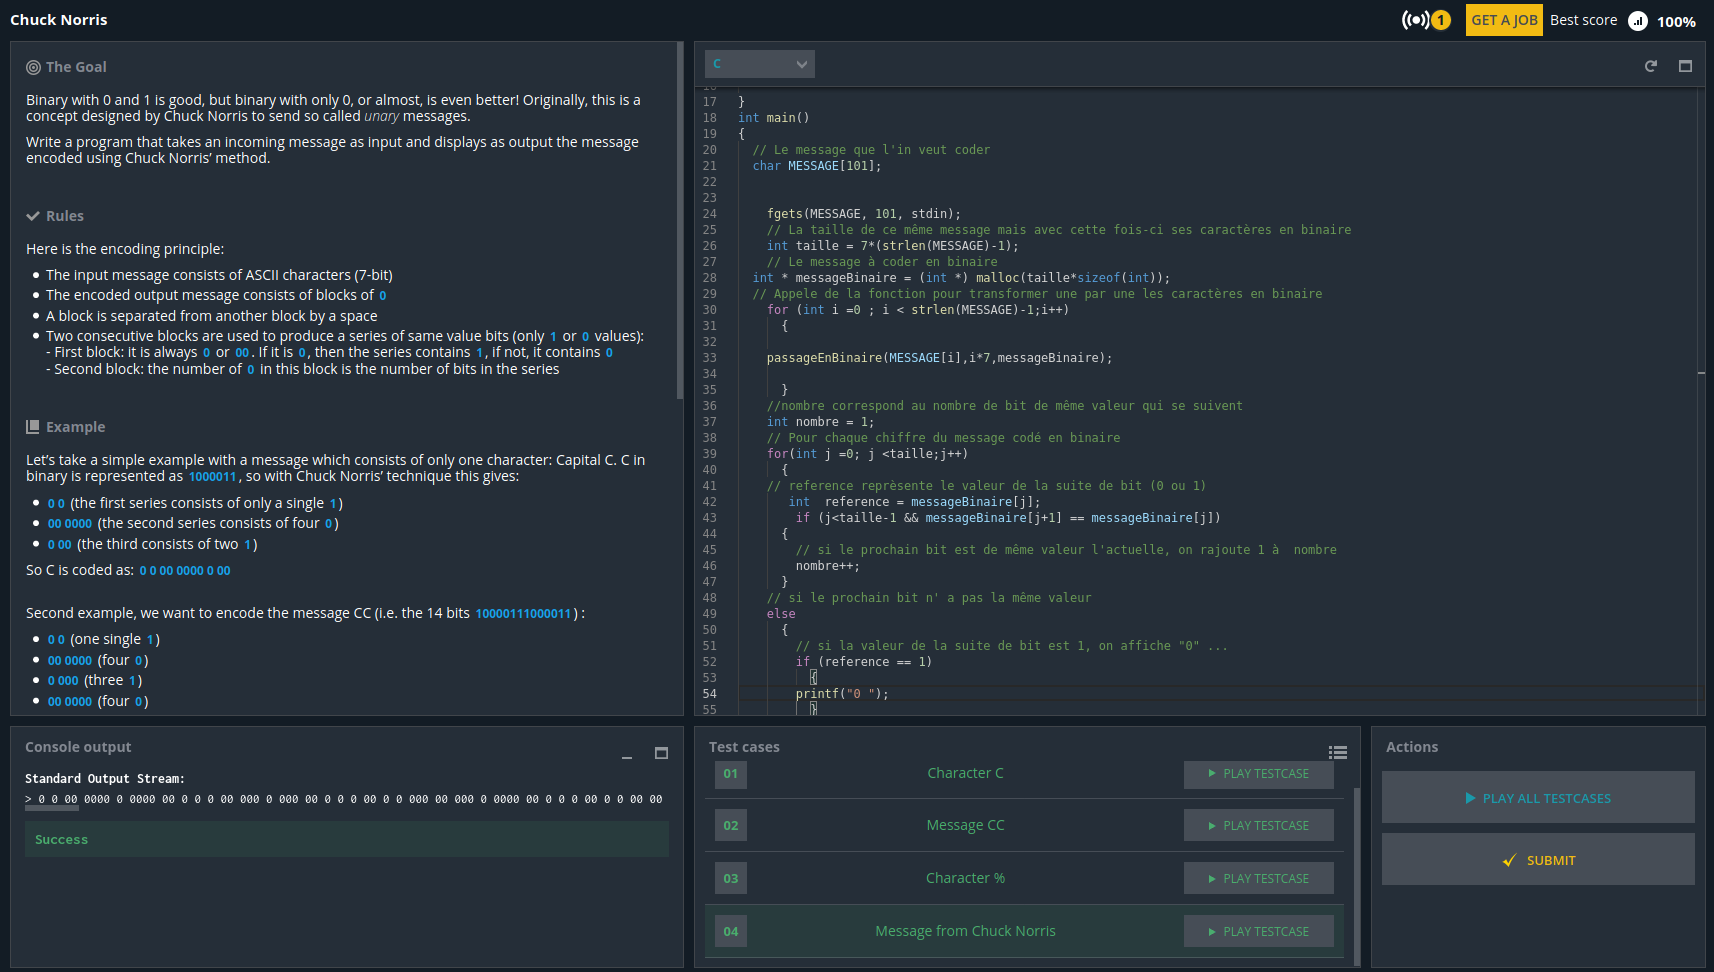
\includegraphics[width=.9
      \linewidth]{./img_rapport/img_coding_game.png}
      \caption{Le site de codingGame.}
      \label{fig-coding-game}
 \end{figure}


 \begin{multicols}{2}
   Le but serait donc d'avoir sur la partie gauche une zone pour entrer les
   informations et sur la droite tout ce qui concerne l'affichage des
   résultats ainsi que certaines informations.

   La partie gauche contiendra donc forcément une balise \texttt{textArea}
   servant à rentrer notre code à tester et une balise \texttt{input}
   permettant à l'utilisateur de rentrer l'identifiant de l'exercice pour
   lequel il soumet une solution.

   Dans la partie droite, nous souhaitions afficher un paragraphe donnant de
   brèves indications sur le fonctionnement du site, ainsi qu'un bouton et une
   zone de texte permettant la soumission du code et l'affichage des résultats
   des tests. Pour cela le bouton doit appeler une fonction JavaScript que l'on
   verra plus tard. Une idée qui nous est venue un peu plus tard fut la mise
   en place d'un autre bouton afin d'obtenir des informations sur le test
   actuel. Ce bouton doit aussi appeler une fonction JavaScript qui agit de la
   même manière que le bouton pour envoyer le code.

   Une fois une idée assez grossière de la composition de notre site, on s'est
   attelé à sa création. En travaillant sur la structure du site, nous nous
   sommes rendu compte que la partie gauche était beaucoup trop chargée en
   informations et texte et que cela nuisait à sa lisibilité. Nous avons donc
   décidé d'implémenter un système d'onglets en utilisant JavaScript pour
   faire de l'affichage dynamique. Cette nouvelle fonctionnalité nous a forcé
   à modifier notre page HTML ainsi que le CSS  en cours de route mais le
   résultat obtenu était beaucoup plus satisfaisant. Cependant ce dernier sera
   expliqué plus loin. Le HTML n'est pas ce qui nous a pris le plus de temps
   car malgré un début compliqué dû à notre méconnaissance de ce langage, il
   est assez rapide à prendre en main et nous n'avions pas besoin de beaucoup
   de pratique pour réaliser notre objectif. Néanmoins, il nous à fallu
   plusieurs essais pour obtenir un résultat satisfaisant. De plus le code CSS et
   certaines parties du code JavaScript nous ont forcés à réécrire notre code. Au
   final, notre organisation en système d'onglet nous a permis de regrouper
   toutes les parties du site en une seule page HTML stockée dans le fichier
   \texttt{index.html}.
 \end{multicols}

  \subsubsection{Explication du code}

  Le document \texttt{index.html} est composé des balises de base pour tout
  document HTML tel que le \texttt{<DOCTYPE >}, \texttt{<html>},
  \texttt{<meta>}, \texttt{title}, \texttt{<head>} et \texttt{<body>}.  On
  ajoute aussi dans la balise \texttt{header} cette ligne :

  \begin{lstlisting}[language=HTML5]
    <link rel="stylesheet" href="./style.css" type="text/css"/>
  \end{lstlisting}

  Qui va permettre d'afficher la mise en forme \texttt{CSS} défini dans notre
  fichier \texttt{style.css} que nous détaillerons dans la partie dédiée.

  Il y aussi juste au dessus une ligne très similaire mais qui elle permet de
  charger \texttt{base.css}. Cette stylesheet réinitialise toutes les balises
  utilisées afin d'avoir le même résultat sur tout les navigateurs. En effet
  d'un navigateur web à l'autre, les mises en forme de base peuvent changer et
  si on ne les redéfinie pas dans le CSS il peut arriver que les paramètres par
  défaut entrainent des problèmes dans la mise en page.

  On va ensuite avoir 2 balises \texttt{div} afin de séparer les parties
  gauche et droite de l'écran avec la première contentant de quoi entrer le
  code et la seconde le reste comme dit précédemment. Elles auront comme
  identifiant \texttt{left-panel} et \texttt{right-panel}. Dans la première on
  va ajouter un \texttt{TextArea} pour accueillir le code de l'utilisateur:

  \begin{lstlisting}[language=HTML5]
    <textarea spellcheck="false" id="code-input" class="code-input"
                              name="code" cols="100" rows="40">Put your code here!</textarea>
  \end{lstlisting}

  Juste après, un autre \texttt{textarea} plus petit va permettre d'ajouter une
  fonctionnalité définit en JavaScript mit au point lorsque qu'on s'entraînait.
  Celui-ci indique juste le nombre de lignes, de mots et
  de caractères qu'on à écrit dans le \texttt{textarea}. On a décidé de le laisser.

  Ensuite on a un autre \texttt{input} afin que l'utilisateur puisse entrer
  l'identifiant de son programme:

  \begin{lstlisting}[language=HTML5]
    <input type="text" id="exercise-id" name="Exercice ID" required />
  \end{lstlisting}

  On a ainsi tous les éléments composant la partie gauche de l'écran.

  En ce qui concerne la partie droite, elle a beaucoup été modifiée suite à la
  partie JavaScript, notamment par l'ajout d'onglet. On va juste s'intéresser à
  cette partie une fois les onglets implémentés car c'est elle qui est restée dans le résultat
  final.

  Dans un premier temps on a une liste de balise \texttt{<a></a>} qui vont
  servir pour changer d'onglets, elles correspondent sur la page au bouton
  contrôlant les panels. Ces dernières vont à chaque fois qu'elles sont
  activées, lancer une fonction JavaScript que nous détaillerons plus tard.
  Ensuite on va avoir nos onglets et leur contenu dans des \texttt{div}. En
  effet se ne sera pas notre JavaScript qui va générer les panels en fonction
  des clics, ce dernier va juste s'occuper de cacher ou faire apparaître le
  panel que l'on désire voir. Un exemple de panel:

  \begin{lstlisting}[language=HTML5]
    <div id="panel0" class = "tabContent">
    <h2>INSTRUCTIONS</h2>
    <h3>Fonctionnement du site</h3>
    <p class="paragraphe-instructions">
    Ce site web est destiner à tester vos réponce aux différents exercices
    donnés par vôtre professeur. <br /> Utilisez le bouton en haut à gauche de
    la page pour faire défiler les différents menus qui seront afficher sur la
    partie droite de vôtre écran.<br />
    </p>
    <h3>Lancement des tests</h3>
    <p class="paragraphe-instructions">
    <ol>
    <li>Collez vôtre code réponce dans la zone de texte prévue à cet effet.</li>
    <li>Entez l'identifiant du jeux de tests à utiliser.</li>
    <li>Cliquez ensuite sur le bouton <strong>"Lancer les tests"</strong>.</li>
    </ol>
    </p>
    </div>
  \end{lstlisting}

  Enfin on finit en appelant justement les différents scripts JavaScript dont on
  a besoin. Ces appels sont à la fin pour être sûr que tout nos éléments HTML
  soient définis, permettant ainsi d'éviter de potentiels erreurs si JavaScript
  tente d'interagir avec un élément qui n'a pas chargé. Cela permet aussi
  d'éviter que rien ne s'affiche si JavaScript ne charge pas correctement.

\subsection{La mise en forme : le CSS}
  \label{subsec:css}

  Le CSS a été écrit parallèlement au HTML, en effet lorsqu'on modifiait le
  format de notre page web, certain éléments ne semblaient pas à leur place, On
  a donc pendant longtemps tâtonné et modifié des éléments mineurs pour obtenir
  un résultat satisfaisant.

  \subsubsection{Explication du code}

  L'un des premiers objectif était la mise en forme des parties gauche et
  droite de la page, pour qu'elles soient notamment à la bonne position. Cela
  est rendu possible avec le CSS via les attributs \texttt{justify-content} et
  en fixant leur taille à 50\% de la taille du document (\texttt{width}). Il
  vaut mieux préférer les pourcentages (positionnement relative) aux valeurs
  absolues comme px, cm ou encore mm (positionnement absolue) afin d'avoir une
  mise en forme ajustable en fonction de la taille de la fenêtre.  Cela permet
  une meilleur compatibilité avec n'importe quel type d'écran ainsi que de
  donner à l'utilisateur la possibilité d'ajuster sans problèmes la taille de
  notre site. Le reste des attributs dans les sélecteurs pour notre partie
  gauche et droite sont surtout là pour la couleur, ici la couleur de fond
  (\texttt{background-color}) et avoir des espacements plus marqués
  (\texttt{margin}).

  \begin{lstlisting}[language=CSS]
    div.left-panel {
      justify-content: left;
      margin-right: 30px;
      margin-left: 100px;
      margin-bottom: 25px;
      background-color: #ffffff;
      box-shadow: 0 1px 6px 0 rgba(32, 33, 36, 0.28);
      width: 50%;
    }


    div.right-panel {
      justify-content: right;
      margin-right: 100px;
      margin-bottom: 25px;
      background-color: #ffffff;
      box-shadow: 0 1px 6px 0 rgba(32, 33, 36, 0.28);
      width: 50%;
    }
  \end{lstlisting}

  Il nous a aussi fallu mettre en forme les éléments de base tel que le
  \texttt{body}, les \texttt{header}\dots Afin d'avoir les plus gros éléments
  composants la page avec un format plus attrayant de celui de base. On a donc
  pour le body des attributs pour modifier ses marges et lui donner une couleur
  plus visible.

\begin{lstlisting}[language=CSS]
  body {
  background-color: #e7e9eb;
  padding: 0 0 0 0;
  margin: 0;
}
\end{lstlisting}

Le header suit la même logique à quelques variations près, notamment l'ajout
d'une \texttt{box-shadow}

\begin{lstlisting}[language=CSS]
header {
  position: relative;
  width: 100%;
  background-color: #1E2127;
  text-align: center;
  padding: 0 0 0 0;
  height: 60px;
  margin-bottom: 25px;
  box-shadow: 0 1px 6px 0 rgba(32, 33, 36, 0.28);
}
\end{lstlisting}

On a aussi modifié les titres de premier et second niveaux, notamment en
changeant la couleur de leur texte, la couleur de fond et leur police.

\begin{lstlisting}[language=CSS]
header h1 {
  margin-top: 0;
  color: #ffffff;
  background-color: #1E2127;
  padding: 5px 0 0 0;
}


h2 {
  text-decoration: underline dotted;
  margin-left: 10px;
}
\end{lstlisting}

Les autres éléments importants à modifier étaient les inputs, contenu en
majorité dans le panel gauche. Comme pour les autres éléments HTML qu'on a vu
avant, ce qu'on a surtout modifié c'est leur couleur, leur taille, ou leur
position ainsi que leurs marges ou bordures. A noter que pour leur taille on
utilise toujours \texttt{width} avec des pourcentages afin de garder un aspect
dynamique. Il y a aussi l'apparition de l'attribut \texttt{max-width} afin
d'éviter que notre \texttt{textarea} ne dépasse la taille de notre panel gauche
à force de modifier la taille de la fenêtre.

\begin{lstlisting}[language=CSS]
div.code-input {
  display: block;
}


textarea {
  background-color: #282c34;
  color: #bbc2cf;
  margin-left: 5%;
  max-width : 90%;
  line-height: 1.5;
  border-radius: 5px;
  border: 1px solid #ccc;
  box-shadow: 1px 1px 1px #999;
}


div.id-input {
  display: table-cell;
  margin-left:auto;
  margin-right:auto;
  width: 65%;
}


div.result-frame {
  background-color: #557883;
  margin: 10px;
}
\end{lstlisting}

La partie qui suit a été rajouté lorsqu'on a voulu implémenter la notion
d'onglets dans notre page web. En effet il fallait mettre en forme et modifier
le positionnement des boutons pour changer d'onglets. On a d'abord cherché à
utiliser des balise \texttt{button} cependant, celle-ci n'étant pas adaptées
elles étaient très compliquées à manipuler et à positionner et on a finalement
décidé d'utiliser une liste de liens. Chacun des éléments de la liste possède
un fond noir qui devient blanc lorsqu'on passe la souris dessus, c'est une
méthode très utilisée dans beaucoup de sites qui rend l'utilisation des boutons
simple et intuitive (si un utilisateur passe la souris sur un élément qui
change aussitôt de couleur, il sait par habitude que c'est un élément avec
lequel il peut interagir en cliquant dessus).

\begin{lstlisting}[language=CSS]
.tab {
  overflow: hidden;
  border: 1px solid rgb(0, 0, 0);
  background-color: #5578FF;
}

.tab ul {
  display: flex;
  justify-content: center;
  list-style-type: none;
  text-align: center;
  width; 100%;
  margin: 0;
  padding: 0;
}

.tab li {
  display: table-cell;
  background-color: black;
  width: 33.5%;
  margin: 0;
  padding: 0;
  outline: none;
  cursor: pointer;
  font-size: 17px;
  font-family: Arial, Helvetica, sans-serif;
}

.tab li:hover {
  background-color: #ffffff;
}

.tab li:active {
  background-color: #ccc;
}

.tab li a {
  color: white;
  text-decoration: none;
  margin: 0;
}

.tab li:hover a {
  color: black;
}
\end{lstlisting}

De même il fallait cacher les panels non voulus avec l'attribut
\texttt{display:none} et les mettre en forme.


\begin{lstlisting}[language=CSS]

.tabContent {
  display: none;
  padding: 10px 10px 10px 10px;
  border: 1px solid #ccc;
  width: 90%;
  height: 90%;
  margin-bottom: auto;
  margin-top: 3%;
  margin-left: auto;
  margin-right: auto;
  max-width : 90%;
  max-height : 90%;
\end{lstlisting}

Il y a aussi d'autres éléments qu'on a modifié mais il sont très similaires à
d'autres présents ici.

Pour finir voici 2 mises en formes différentes de notre site, la première est
une des toutes premières versions et la seconde celle que l'on peut voir
actuellement.

  \begin{figure}[htbp]
    \centering
    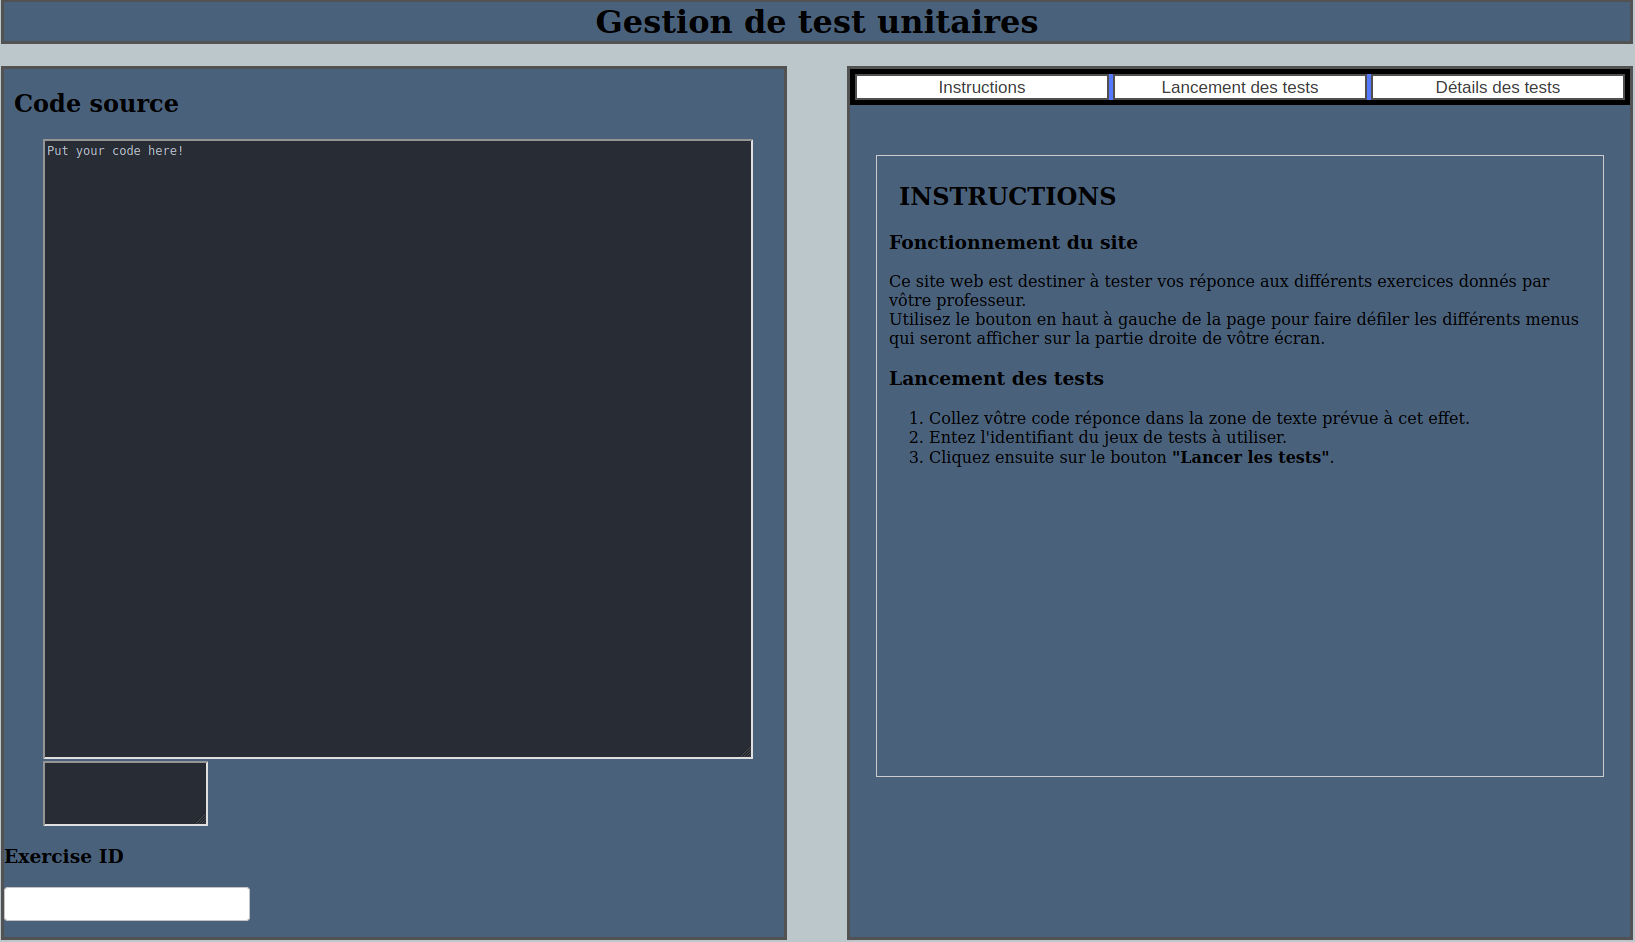
\includegraphics[scale=0.25]{./img_rapport/page_web_v1.png}
    \caption{Un des tout premiers résultat satisfaisant}
    \label{fig-page-web-v1}
  \end{figure}


  \begin{figure}[htbp]
    \centering
    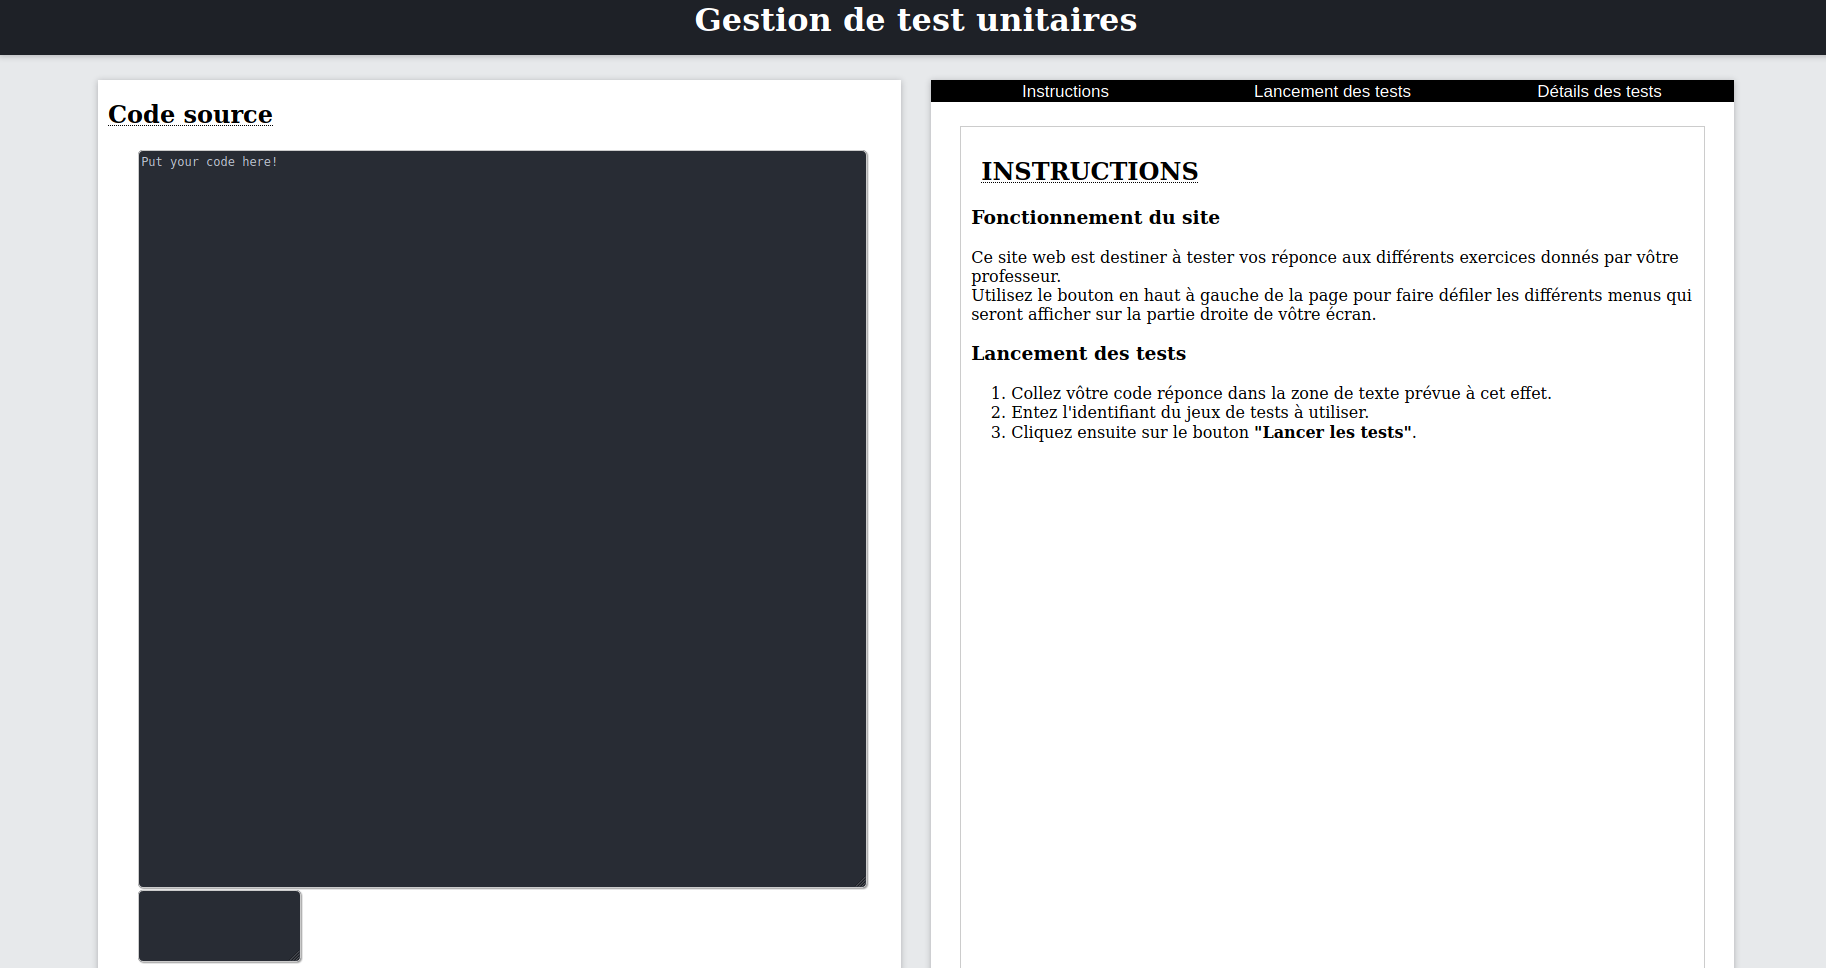
\includegraphics[scale=0.25]{./img_rapport/page_web_v2.png}
   \caption{Le résultat final}
   \label{fig-page-web-v2}
 \end{figure}

\newpage
\subsection{Un peu de dynamisme côté client : JavaScript}

Le JavaScript sert à deux choses dans notre page web:
\begin{itemize}
\item Apporter quelque fonctionnalités intéressantes que l'HTML ou le CSS ne
  peuvent pas faire. Ce qui concerne les onglets et un compteur de caractères,
  mots et lignes.
\item La liaison entre notre côté client et le serveur, qui est une partie très
  importante car c'est via cette liaison qu'on va pouvoir communiquer avec la
  base de données et traiter le code des utilisateurs.
\end{itemize}

\subsubsection{Premier cas : panel.js}

L'un des premiers ajout assez simple fut le compteur de lignes, mots et
caractères. Cette fonctionnalité n'était en aucun cas indispensable, cependant
elle nous a permis de nous familiariser avec JavaScript avec un exemple
concret (notamment la gestion des événements).

\begin{lstlisting}[language=JS]
// Fonction pour indiquer le nbr de ligne,mot,lettre.
code.addEventListener('input', function (e) {
    e.stopPropagation();
    let compt_line = code.value.substr(0, code.selectionStart).split("\n").length;
    let compt_word = compt_line + code.value.substr(0, code.selectionStart).split(" ").length - 1;
    text_pos.value = "line :" + compt_line + "\nword :" + compt_word + "\nchar :" + code.value.length;
});
\end{lstlisting}

Cette fonction va être appelée chaque fois que l'utilisateur écrit dans le
\texttt{textArea} contenant le code, pour cela on utilise un
\texttt{addEventListener} qui prend en argument notre \texttt{event}. On va
devoir exécuter dans cette dernière la fonction donnée en arguments. Cette
fonction va regarder la string présente dans le \texttt{textArea} puis il nous
suffit de compter le nombre de retours chariot (\texttt{\textbackslash n}) pour
avoir le nombre de lignes, le nombre de mots correspond de façon similaire au
nombre d'espace plus le nombre de lignes, enfin pour le nombre de caractères il
suffit juste de calculer la taille de la chaîne. Il faut ensuite afficher
dans les éléments HTML voulus le résultat sous forme d'une petite phrase.

L'autre grande fonctionnalité dans notre fichier est la gestion des panels, qui
se fait assez facilement mais qui donne un résultat bien plus propre pour la
page web. Cependant il à fallut modifier aussi bien le HTML que le CSS pour
inclure cette notion d'onglets comme expliqué dans les deux parties
précédentes. Notre script va juste s'occuper d'afficher le bon panel et de
rendre les autres invisibles. Toute la partie texte se trouve dans le HTML et
toute la partie forme dans le CSS.

\begin{lstlisting}[language=JS]
// Fonction qui va afficher/cacher les onglets.
function changementPanel(panel)
{

   for (let g of tabContent) {
        g.style.display = "none";
    }

    document.getElementById(panel).style.display = "block";
}
document.getElementsByClassName("defaultOpen")[0].click();

\end{lstlisting}

Notre fonction va s'occuper de cacher tous les panels dans notre scène, puis
d'afficher celui ayant la même classe que l'argument donné. Celle si sera
appelée lorsqu'on appuie sur l'un des boutons de notre code HTML (du coup on a
pas de \texttt{addEventListener}, c'est HTML qui va appeler cette fonction si
il en a besoin). On à aussi dans notre document HTML un panel avec comme classe
\texttt{defaultOpen} qui va nous permettre lorsque un utilisateur télécharge la
page de déjà afficher un panel.


\subsubsection{Second cas : script.js}

Ce script gère tous ce qui à un lien avec la communication entre client et
serveur. Et ceux en majorité à l'aide de la fonction \texttt{fetch} (sucre
sytaxique pour faciliter l'utilisation de \texttt{XMLHttpRequest}). Pour ce qui
concerne l'envoi de notre code (\texttt{recupCode}), il se divise en 3 requêtes
vers notre serveur. La première va demander un identifiant afin qu'il puisse retrouver
le résultat de son code sans problèmes à l'intérieur de la base de données (dans
l'éventualité où plusieurs résultats sont mis en même temps dans la base). La
seconde va poster notre code ainsi que son tout nouveau identifiant au serveur
afin qu'il puisse la stocker dans la base de données et l'analyser par la suite.
Et enfin la troisième et dernière requête va récupérer le résultat de notre
code traité au bout d'un certain temps et l'afficher.

Pour simplifier les URL sur lesquelles on va envoyer nos requêtes, on utilise
une variable globale \texttt{path} indiquant le chemin vers le dossier
\texttt{tests\_unitaires} contenant tout notre travail. En effet si on connait
le chemin menant à ce dossier là, on peut appeler n'importe quel fichier de
notre projet. Ce qui permet de ne modifier qu'une seule variable lorsqu'on
change de serveur afin qu'il soit toujours fonctionnelle.

\paragraph{Requête pour obtenir un identifiant}

L'identifiant va être obtenu à l'aide d'une requête \texttt{HTTP} \texttt{GET},
en effet c'est le serveur qui génère l'identifiant et la récupéreration de
données se fait bien avec une requête \texttt{GET} Pour cela on va appeler le
code défini ci-dessous.

\begin{lstlisting}[language=JS]
  // get a user id:
  async function  getId()
  {
    let code = document.querySelector('#code-input');
    // test id
    let id_exercice = document.querySelector('#exercise-id');

    return fetch(path+"php/get_id.php")
    .then((response) => response.json())
    .then(response => {
      user_id = response;
      console.log("GET ::: " + response);
    })
    .catch(error => {
      console.log("getIDError:" + error);
    })
  }
}
\end{lstlisting}

Cette fonction est la plus basique des trois. On va effectuer la requête sur un
script \texttt{PHP} nommé \texttt{get\_id} (qui sera expliqué comme tous les
autres script PHP suivant dans leur partie dédiée (voir \ref{php})). La réponse
fourni par ce script est au format \texttt{JSON}, on va donc appeler une
première \texttt{promise} pour transformer notre réponse au format
\texttt{JSON} en entier. Ensuite on va utiliser une autre \texttt{promise} pour
stocker cet identifiant dans une variable global de notre script. On en profite
aussi pour afficher un message sommaire dans la console, ce qui est utile pour
vérifier que les requêtes sont correctement effectuées.

Il faut bien noter que notre fonction contient le mot clé \texttt{async}. En
effet on le verra par la suite mais il important que cette requête soit
\texttt{await} car cela n'a aucun sens de commencer les requêtes suivantes sans
posséder l'identifiant.

\paragraph{Requête pour envoyer notre code au serveur}

Cette fonction va utiliser la méthode \texttt{POST} afin d'envoyer nos
informations (c'est à dire notre code ainsi qu'un identifiant pour savoir à
quel tests il se rapporte) au serveur.

\begin{lstlisting}[language=JS]

    async function getCode()
{
    return fetch(path+"php/get_code.php", {
        method: 'post',

	body: JSON.stringify({"user_id": user_id, "id_exercise": id_exercice.value, "code": code.value}),
        headers: {
            'Content-Type': 'application/json'}
    })
        .then(function (resp) {
            console.log("REPONSE ::: ", resp)
        })
        .catch(function (err) {
            console.log("ERROR ::: ", err)
        })
}
\end{lstlisting}

La requête \texttt{POST} et un peu différente des \texttt{GET}, les
informations à envoyer sont contenu dans le \texttt{body} de la requête. On à
décidé dans notre cas d'envoyer nos données sous la forme \texttt{JSON}. Il
faut aussi rajouter quelques informations à notre requête notamment le fait
que ce soit un \texttt{POST} ou encore que les informations transmis sont sous
le format \texttt{JSON} (défini dans le \texttt{headers}).

On va ensuite afficher la réponse obtenu mais seulement dans le but de voir
l'état de notre requête, en effet vu que c'est un \texttt{POST} aucun retour
n'est attendu normalement.

Le mot clé \texttt{async} et aussi très important dans cette fonction car on ne
peut pas obtenir de réponse si notre code n'a même pas encore été reçu et
traité par notre serveur.

\paragraph{Requête pour recevoir notre résultat au code envoyé}

La dernière requête appelée va être celle permettant de récupérer le résultat
de notre code suite aux tests exécutés côté serveur. Pour cela on va utiliser
une méthode \texttt{GET} (cependant il y a modification des données côté
serveur, ce qui est contradictoire avec le fait que la requête \texttt{GET}
doit respecter le principe d'idempotence et être sans effets de bord comme on va
le voir ici [\ref{sub:get-result}], mais nous ne savions pas quel autre requête
utiliser). Cette fonction va être très similaire à \texttt{getID}, à la seule
différence notable que l'on va envoyer via l'URL l'identifiant de notre code
(voir ci-dessous).

\begin{lstlisting}[language=JS]
 var urlResult = path+"php/get_result.php?user_id=" + user_id;
\end{lstlisting}

Les deux autres différences sont juste que notre réponse n'est pas sous le
format \texttt{JSON} et il donc inutile de le transformer. De plus la réponse
doit être affichée non pas dans la console mais dans l'élément \texttt{HTML}
prévu à cette effet.


\begin{lstlisting}[language=JS]
// get the result of our code
async function getTest()
{
    var urlResult = path+"php/get_result.php?user_id=" + user_id;
    await fetch(urlResult).then(data => {
        console.log("GET ::: ", data);
        data.text().then(function (text) {

            document.querySelector('#result-output').innerText = text;
        });
    }).catch(error => {
        console.log(error);
        document.querySelector('#result-output').innerText = error;
    })
}
\end{lstlisting}

Une fois cette requête et ses \texttt{promise} terminées, notre page devrait
afficher le résultat du tests de notre code (dans le cas ou aucune erreur n'est
apparu).

\paragraph{Rassemblement des ces trois fonctions}

Pour avoir le résultat escompté lorsqu'on clique sur le bouton, il suffit donc
d'appeler à la suite ces trois fonctions (en n'oubliant pas d'enlever le fait
qu'elles sont asynchrones de base).

\begin{lstlisting}[language=JS]
async function recupCode() {
    if(document.getElementById('exercise-id').value != "")
    {
        await getId();
        await getCode();
        setTimeout(getTest,2000);
    }
}
\end{lstlisting}

\texttt{get\_test} ne peut se lancer que lorsque notre requête dans
\texttt{get\_code} est fini, c'est à dire lorsque le serveur reçoit nos
informations. Cependant on ne peut pas être sûr qu'elle soit traitée et
analysée dans la foulée, on à donc préféré attendre deux seconde afin de bien
laisser le temps au serveur de traiter notre code.

\\

Voici comment se déroule la communication entre JavaScript et php lorsque
l'utilisateur appui sur le bouton pour lancer les tests:

\\

\begin{figure}[htbp]
  \centering
  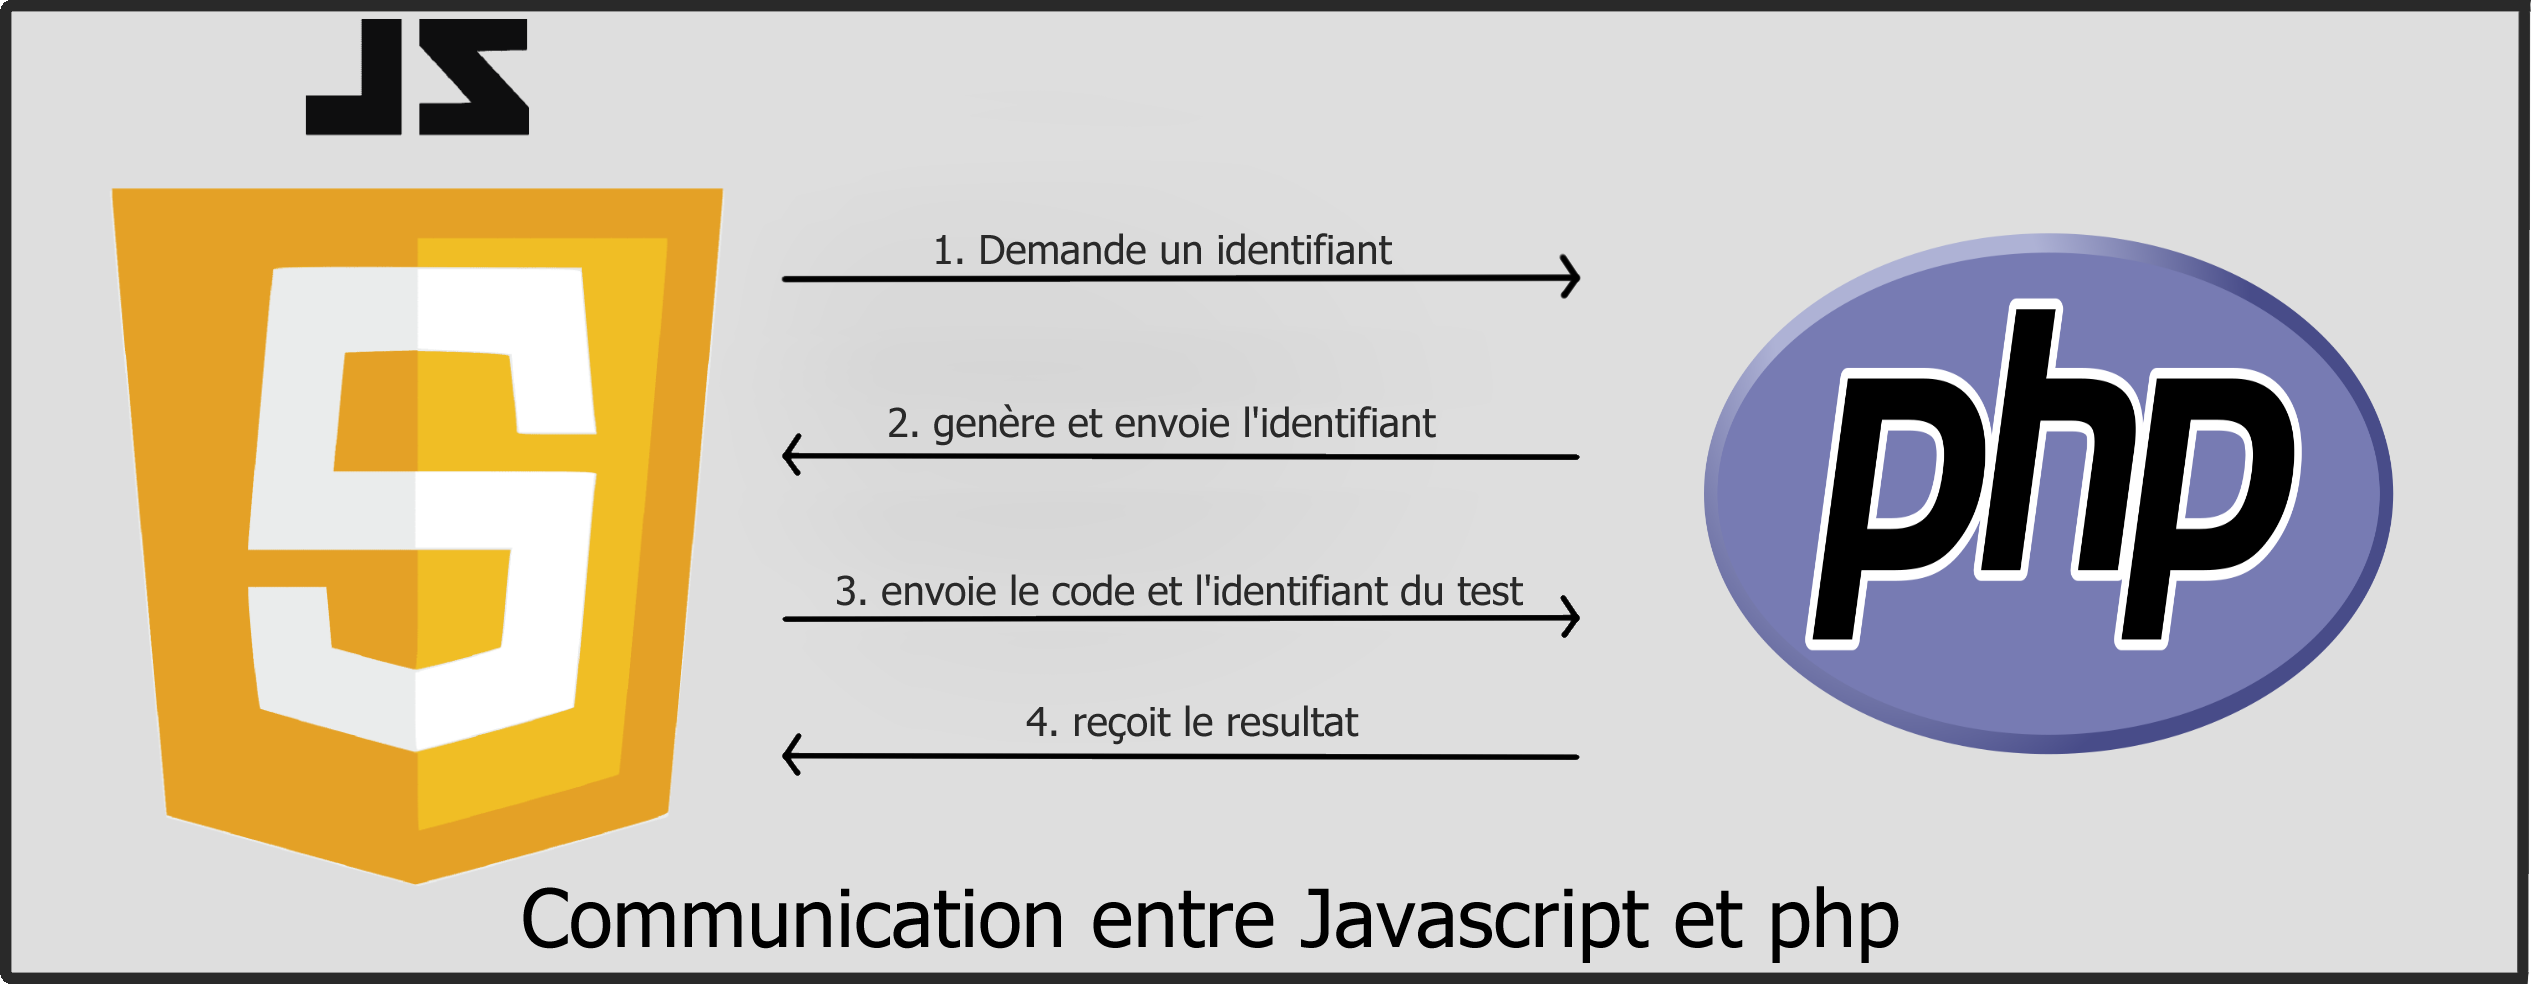
\includegraphics[scale=0.16]{./img_rapport/shema_com_js_php.png}
  \caption{Communication entre JavaScript et php}
  \label{fig-page-web-v1}
\end{figure}


\subsubsection{Une autre requête : obtenir des informations}
\label{subsec:getInfo}

On a aussi un bouton sur notre page pour avoir plus d'informations et de détails
sur les tests. Cette fonction utilise le même principe que \texttt{getTest}.

\begin{lstlisting}[language=JS]
function displayTestsDetails() {
    var urlInfo = path+"php/get_info.php?id_exercise=" + id_exercice.value;
    fetch(urlInfo).then(response => response.text()).then(data => {
        console.log(data);
        document.querySelector('#test-details').innerText = data;
    }).catch(error => {
        console.log(error);
        document.querySelector('#test-details').innerText = error;
    })
}
\end{lstlisting}

\section{Côté serveur : PHP python et SQL}
\label{sec:serveur}

\subsection{Le lien entre les deux, le PHP}
\label{sec:PHP}

Dans notre projet, php va servir seulement pour recevoir les requêtes
effectuées par le côté client grâce au JavaScript avec \texttt{fetch} et aux
différentes actions à mener en fonction de ces requêtes. Pour cela on a divisé
les tâches en 4 grandes parties, chacune traitée dans un script différents.

Pour pouvoir envoyer des requêtes en PHP à la base de données on utilise
l'extension \texttt{PDO}.

Le PHP était aussi un langage totalement inconnu pour nous deux et ce projet
nous à permit d'en avoir un avant goût.

\subsubsection{Obtention d'un ID (script get\_id)}
\label{sub:get-id}

Notre client va envoyer son code au serveur qui va donc être stocké dans la
base de données, cependant comme décrit plus loin il va falloir se rappeler
quel est son code pour pouvoir lui renvoyer la réponse adéquate. Pour cela on
va lui donner une ID (un entier) compris entre 1 et 10000 \emph{unique} (dans
le cas ou le site devrait avoir à interagir avec plus de 10000 utilisateurs, on
peut augmenter ce nombre ou même utiliser une suite de caractères
alphanumériques). Pour cela la méthode utilisée consiste à obtenir de façon
aléatoire un entier, et ensuite on regarde si il n'existe pas une ID
équivalente dans la base de données, si il n'y en a pas alors notre ID est bien
\emph{unique} et il nous suffit alors de \texttt{echo} de notre ID (ce qui va
être echo est ce qui va être reçu par fetch en réponse). Dans l'autre cas on
recommence l'étape jusqu'à ce que l'ID soit bonne. Dans le cas où tous les ID
possible sont utilisés (ce qui est très peu probable mais possible). Notre
boucle va être infini, cependant on réalise la requête à chaque tour, ainsi
notre script python peut entre temps libérer une ID, la rendant disponible. Une
fois notre ID pour le client trouvée on prépare la base de données à recevoir un
code avec cette ID, ainsi, si une requête est effectuée dans la foulée par un
autre utilisateur il n'aura pas la possibilité de prendre la même ID.

\begin{lstlisting}[language=PHP]
  <?php
    #header("Access-Control-Allow-Origin: *");
    #header("Content-Type:application/json");

    function isIN($\dollar$newID, $\dollar$ids) {
      while($\dollar$id = $\dollar$ids->fetch()) {
        if ($\dollar$newID == $\dollar$id['idProgramme']) {
          return true;
        }
      }
      return false;
    }

    # Getting current used id list
    $\dollar$myPDO = new PDO("sqlite:../db/sql/tests_unitaires.db");
    $\dollar$newID;

    # Generating new id
    do {
    $\dollar$ids = $\dollar$myPDO->query("SELECT id_programme FROM programme_utilisateur;");
      $\dollar$newID = random_int(0, 10000);
    } while (isIN($\dollar$newID, $\dollar$ids));

    # Adding newID to db:

    $\dollar$request = $\dollar$myPDO->prepare("INSERT INTO programme_utilisateur(id_programme,
      code, test) VALUES (?, NULL, NULL)");
    $\dollar$request->execute(array($\dollar$newID));
    echo $\dollar$newID;
  ?>
\end{lstlisting}

\subsubsection{Stocker le code dans la base de donnée (script get\_code)}
\label{sub:get-code}

Une fois l'ID obtenu pour le code et une place réservée dans la base de
données.  Il reste encore à stocker le code ainsi que l'identifiant du test. On
va donc devoir dans un premier temps récupérer ces deux variables et pour cela
un problème s'est posé: en effet normalement toute information fournie via une
requête HTTP \texttt{POST} peut être récupérée en PHP à l'aide de la variable
spéciale \texttt{\$\_POST}. Cependant, l'information transmise
sous le format \texttt{JSON} n'est pas placée dans cette variable,
il faut donc la décoder pour pouvoir l'utiliser.
Une solution à ce problème fut d'utiliser ce bout de code ci-dessous.

\begin{lstlisting}[language=PHP]
  <?php

    header("Access-Control-Allow-Origin: *");
    header("Content-Type:application/json");

    $\dollar$personalPost = json_decode(file_get_contents('php://input'),true);

    $\dollar$userID = $\dollar$personalPost['user_id'];
    $\dollar$exerciseID = $\dollar$personalPost['id_exercise'];
    $\dollar$code = $\dollar$personalPost['code'];

  \end{lstlisting}

Ensuite on réalise une simple requête \texttt{UPDATE} pour ajouter les
variables \texttt{code} et \texttt{exerciseID} dans le tuple de la table

\texttt{programme\_utilisateur}.

\begin{lstlisting}[language=PHP]
    $\dollar$myPDO = new PDO('sqlite:../db/sql/tests_unitaires.db');
    $\dollar$request = $\dollar$myPDO->prepare("UPDATE programme_utilisateur SET code = ?, test
      = ? WHERE id_programme = ?;");

    $\dollar$request->execute(array($\dollar$code,$\dollar$exerciseID,$\dollar$userID));
  ?>
\end{lstlisting}

\subsubsection{Obtenir les résultats (script get\_result)}
\label{sub:get-result}

Ce script va aussi s'exécuter en deux temps. Lorsqu'on va appeler ce script il
va tout d'abord nous renvoyer le résultat du test stocké dans la base de
données, plus précisément dans la table \texttt{retour} (qui sera remplie via le
script python que nous détaillerons plus tard). Pour cela on va de la même
manière qu'avant faire une requête \texttt{SQL} avec \texttt{PDO} en précisant
que l'on veut le tuple avec notre identifiant fourni par \texttt{get\_id}.
Pour récupérer cette identifiant il suffit juste d''utiliser la variable
spéciale \texttt{\$\_GET} de PHP, qui consiste en un tableau contenant chacune
des informations passées à la requête \texttt{HTTP} de tel sorte que la clé soit
le nom de la variable et le résultat le contenu de cette case.

Ensuite une fois qu'on a echo le résultat (c'est à dire que l'utilisateur va
recevoir la réponse à son test) il nous suffira de supprimer celui-ci de la
base de données, afin de libérer la place maintenant inutile et éviter par la
suite de renvoyer ce code si une réponse avec le même identifiant arrive.

\begin{lstlisting}[language=PHP]
  <?php
    ini_set('display_errors', 1);
    ini_set('display_startup_errors', 1);
    error_reporting(E_ALL);

    $\dollar$userID = $\dollar$_GET['user_id'];
    $\dollar$myPDO = new PDO('sqlite:../db/sql/tests_unitaires.db');

    $\dollar$request = $\dollar$myPDO->prepare("SELECT resultat FROM retour WHERE id_utilisateur = :id");
    $\dollar$request->execute(['id' => $\dollar$userID]);

    while($\dollar$res = $\dollar$request->fetch())
    {
        echo str_replace("\\n","\n",$\dollar$res["resultat"]);
    }

    $\dollar$request = $\dollar$myPDO->prepare("DELETE FROM retour WHERE id_utilisateur = :userID;");
    $\dollar$result = $\dollar$request->execute(['userID' => $\dollar$userID]);
  ?>
\end{lstlisting}

\subsubsection{Information sur le test (script get\_info)}
\label{subsec:get-info}

On a aussi intégré un moyen pour l'utilisateur d'avoir directement sur le site
un résumé rapide de ce qui est attendu pour le test (ce résumé doit être écrit
préalablement dans la base de données dans la variable \texttt{info\_test}
présent dans la table \texttt{test}). Ainsi il aura juste à marquer le bon
identifiant du texte dans le \texttt{textarea} prévue à cette effet et cliquer
sur le bouton pour avoir ce résumé.

Pour cela le code php est très similaire à ce qui a été vu précédemment. On récupère
dans la variable spéciale \texttt{\$\_GET} de PHP notre \texttt{id\_exercise}
contenu dans le \texttt{textarea}, puis on effectue une requête à la base de
données pour récupérer la variable contenant le résumé vu plus haut, et enfin on
le retourne avec un echo.


 \subsection{La base de données}%
 \label{sec:La base de données}

  Pour la gestion de la base de données, nous avons décidé d'utiliser
  \texttt{SQLite} car c'est un outil simple d'utilisation que nous avions vue
  dans le cours de base de données enseigné à la fac. Le projet ne nécessitait pas
  de réflexion très aboutie sur la construction du système d'information,
  cependant, nous avons tout de même décidé de créer une base de données assez
  complexe (pour nôtre niveau) pour deux principales raisons. D'une part pour
  simplifier de potentiels ajouts de fonctionnalités plus avancées au site et
  d'autre part, pour approfondir et mettre en pratique ce que nous avions appris
  durant nôtre quatrième semestre.

  \subsubsection{Conception de la base}%
  \label{sub:Conception de la base}


  La construction de la base s'est faite en plusieurs étapes, dès le départ, il
  semblait évident qu'il y avait trois principales informations à stocker. Tout
  d'abord, il y a les \textbf{tests}, le but du site étant de faire de la
  gestion de tests unitaires, cela nécessite un moyen de stocker ces tests,
  ainsi que toutes les informations les concernant comme le langage, la
  commande de compilation ou encore de potentielles informations les décrivant.
  Les deux autres informations à stocker vont de paire puisqu'il s'agit des
  \textbf{programmes à tester} (envoyés via une requête HTTP depuis un
  navigateur) et des \textbf{résultats aux tests}. A la fin de cette première
  étape, nous avons séparé ces trois informations dans trois différentes tables
  \texttt{tests}, \texttt{programme\_utilisateur} et \texttt{retour}.

  Après la création des trois tables décrites ci-dessus, une autre question
  s'est posée à nous: \textit{quels informations devons nous exactement stocker
  dans chacune des tables ?} Pour la table \texttt{programme\_utilisateur}, il
  nous faut un identifiant que l'on a appelé \texttt{id\_programme} qui est la
  \textbf{clé primaire} de la table de type \texttt{TEXT} (nous avons convenu
  que cela était moins restrictif qu'un simple entier). Ensuite, nous avons
  deux autres attributs, \texttt{code} de type \texttt{TEXT} qui correspond au
  code envoyé par l'utilisateur du site et un attribut \texttt{test} qui est
  une \textbf{clé étrangère} correspondant à l'identifiant du test demandé par
  l'utilisateur (lui aussi de type \texttt{TEXT}).

  \begin{lstlisting}[language=SQL]
  CREATE TABLE programme_utilisateur
  (
    id_programme TEXT,
    code TEXT,
    test TEXT,
    PRIMARY KEY(id_programme),
    FOREIGN KEY(test) REFERENCES tests(id_test)
  );
  \end{lstlisting}

  La table \texttt{retour} est identifiée par l'attribut \texttt{idRetour} (
  \texttt{TEXT} ), elle possède un attribut \texttt{resultat} (correspondant au
  résultats des tests) et une clé étrangère \texttt{idUtilisateur}
  correspondant à l'identifiant de la table décrite précédemment.

  \begin{lstlisting}[language=SQL]
  CREATE TABLE retour
  (
    id_retour TEXT,
    resultat TEXT,
    id_utilisateur TEXT,
    PRIMARY KEY(id_retour),
    FOREIGN KEY(id_utilisateur) REFERENCES Utilisateur(id_utilisateur)
  );
  \end{lstlisting}

  Pour la création des attributs de \texttt{tests}, nous avons du commencer par
  étudier l'organisation de la partie serveur du site pour comprendre comment
  les programmes sont stockés et compilés. Nous en avons conclus qu'il était
  important de stocker les commandes de compilation et d'exécution dans les
  attributs \texttt{command\_compilation} et \texttt{command\_execution} qui
  seront utilisés par \textbf{python}. A noter que si un programme est écrit
  dans un langage interprété comme \textit{python} ou encore \textit{haskell}
  (qui peut être compilé et interprété), le champ \texttt{command\_compilation}
  sera vide et \texttt{command\_execution} contiendra la commande pour exécuter
  le programme (par exemple \lstinline{python3 prog.py} pour python ou
  \lstinline{runghc prog.hs} pour haskell). Il faut aussi stocker un chemin
  vers le répertoire qui contient le fichier source du tests (par exemple,
  \texttt{../data/cMaths} qui contient le fichier \texttt{main.c}) dans
  l'attribut \texttt{path\_to\_file} pour les suppressions de fichiers
  temporaires comme les fichier de code sources qui contiennent le code de
  l'utilisateur du site ou les fichiers binaires. Cette table possède aussi
  trois autres attributs, \texttt{id\_test} qui est la clé primaire de la table,
  \texttt{info\_test} qui contient une description du test passé (et qui peut
  être \texttt{NULL}) et \texttt{langage} qui correspond à l'extension de
  fichier du langage ( \textbf{py} pour python par exemple  ).

  \begin{lstlisting}[language=SQL]
  CREATE TABLE tests
  (
    id_test TEXT,
    langage TEXT,
    command_compilation TEXT,
    command_execution TEXT,
    nom_compilation TEXT,
    nom_execution TEXT,
    path_to_file TEXT,
    info_test TEXT,
    PRIMARY KEY(id_test)
  );
  \end{lstlisting}

  Cette dernière table a été réécrite plusieurs fois durant le développement du
  script \textbf{python}. En effet, nous avons commencé \textbf{SQL} bien avant
  \textbf{python} et nous ne connaissions pas encore le module
  \texttt{subprocess} utilisé par le script. De plus, certaines fonctionnalités
  ont été apportées durant le développement. Au départ, nous avions pensé le
  site pour gérer des tests unitaires uniquement pour des programmes écrits en
  \textbf{C}, cependant, nous avons jugé plus intéressant et moins restrictif
  que de le rentre compatible avec tous les langages. Ce choix nous a obligé à
  stocker la commande d'exécution dans la table en plus de la commande de
  compilation, pour pouvoir travailler avec des langages exécutés par des
  machines virtuelles comme \textbf{Java}. Il aurait été facile d'utiliser la
  notations \textbf{shebang} pour manipuler des programme écrits dans des
  langages comme python de la même façon que des fichier binaires générés par
  un compilateur( \lstinline{./prog} ), mais cela n'aurait pas été possible
  avec les langages comme \textbf{Java}. Dans le cas de \textbf{Java}, la
  solution aurait été de passer par un script \textbf{shell}, mais cela aurait
  rendu l'utilisation du site beaucoup plus complexe pour la personne qui
  fourni les tests.

  \subsection{Python}%
  \label{sec:Python}

  Pour compiler et exécuter les programmes des utilisateurs du site puis mettre à
  jours la table \texttt{retour} de la base de données, nous avons décidé
  d'utiliser un script python avec les modules \texttt{sqlite3} et
  \texttt{subprocess}. Le module \texttt{sqlite3} permet au programme de se
  connecter à la base de données \textbf{SQLite} de façon similaire à
  \textbf{php} et le module \texttt{subprocess} permet d'exécuter des commandes
  shell et de récupérer leur sortie au format textuel.

  \subsubsection{Intéraction avec SQLite}%
  \label{sub:Intéraction avec SQLite}

  Comme expliqué précédemment, le module \texttt{sqlite3} permet de se
  connecter à la base de données et d'exécuter des requêtes \textbf{sql} de
  façon similaire à php. On utilise la fonction \lstinline{connect()} qui prend
  en paramètre le chemin vers le fichier \textbf{db} (le fichier contenant la
  base de données générée par SQLite) sous forme de chaîne de caractères et
  retourne un objet qui représente la base de données. Pour créer la connexion
  dans le script, on utilise une fonction nommée
  \lstinline{create_connection()}:

  \begin{lstlisting}[language=PY]%
    def create_connection():
        """ Return a connection to the db corresponding to the path given as
        parameter """
        connection = None
        try:
            connection = sqlite3.connect("./sql/tests_unitaires.db")
            #print("connection to SQLite DB successful")
        except Error as err:
            print(f"Connection to DB failed: {err}")

        return connection
  \end{lstlisting}

  Cette fonction retourne la connections vers la base, et en cas de problème,
  affiche le message d'erreur généré par la fonction \lstinline{connect()}.

  Une fois que la connections vers la base de données est créée, il faut générer
  un curseur pour pouvoir exécuter des requêtes. Cela se fait à l'aide de la
  méthode \lstinline{cursor()} de l'objet \lstinline{connection}.

  \begin{lstlisting}[language=PY]%
    connection = create_connection()
    cur = connection.cursor()
  \end{lstlisting}

  L'exécution de requêtes \textbf{sql} se fait alors de la façon suivante:

  \begin{lstlisting}[language=PY]%
    sql_select = """SELECT * FROM programme_utilisateur;"""
    request_result = cur.execute(sql_select).fetchall()
  \end{lstlisting}

  La méthode \lstinline{execute()} prend en paramètre une chaîne de caractères
  contenant la requête et l'exécute. Pour récupérer les données, on peut
  ensuite utiliser les méthodes \lstinline{fetchall()} et
  \lstinline{fetchone()}. Dans l'exemple ci-dessus, on utilise la méthode
  \lstinline{fetchall()} qui retourne un objet itérable qui contient les
  informations extraites. La mise à jours de la base se fait de façon
  similaire, en exécutant une requête de type \lstinline{INSERT} ou
  \lstinline{UPDATE}. A noter que pour que les modifications apportées à la
  base soient sauvegardées, il faut utiliser la méthode \lstinline{commit()} de
  l'objet connections et il faut utiliser la méthode \lstinline{close()} pour
  fermer la connections.


  \subsubsection{Les fonctions intermédiaires}%
  \label{sub:Les fonctions intermédiaires}

  Comme expliqué dans la partie précédente, nous savons maintenant comment
  interagir avec la base de données \textbf{SQLite}. Maintenant, il faut pour
  chaque entrées de la table \texttt{programme\_utilisateur}, effectuer les
  tests et mettre à jours la table \texttt{retour} de la base. Pour cela nous
  avons utilisé une boucle infinie, dans laquelle on vérifie si il y a des
  informations des la table \texttt{programme\_utilisateur}.

  Avant de détailler le ce qui ce passe dans la boucle, commençons par décrire
  les différentes fonctions intermédiaires utilisées dans le script.

  Tout d'abord, nous avons une fonction qui nous permet de récupérer toutes les
  informations sur le test demandé par l'utilisateur du site:

  \begin{lstlisting}[language=PY]%
    def withdrawInformation(id_exercice):
        if id_exercice != None:
            ids = cur.execute("""SELECT id_test FROM tests;""").fetchall()

            l = [i[0] for i in ids]
            if id_exercice in l:
                sql_test = f"""SELECT langage, command_compilation,
                    command_execution, path_to_file, nom_compilation,
                    nom_execution FROM tests WHERE id_test='{id_exercice}';"""
                return cur.execute(sql_test).fetchone()
        return None
  \end{lstlisting}

  Le fonctionnement est le suivant: on commence par sélectionner tous les
  identifiants disponibles dans la table \texttt{tests} à l'aide d'une requête
  SQL et on les met dans une liste.  Si l'identifiant demandé n'est pas valide,
  il ne se trouve pas dans la liste, dans ce cas on met à jour la table retour
  avec un message d'erreur pour faire comprendre à l'utilisateur du site qu'il
  s'est trompé lorsqu'il à écrit l'identifiant du test et on retourne
  \lstinline{None}. Sinon, on récupère toutes les informations utiles comme les
  commandes de compilation et d'exécution et on les retourne sous la forme d'un
  tuple.

  Ensuite, on a une fonction \lstinline{make_test()} permettant de compiler et
  d'exécuter les programmes pour passer les tests.

  \begin{lstlisting}[language=PY]%
    def make_test(code, id_user, id_exercice, path_file, language,
                  command_compilation, command_execution, n_comp, n_exec):

        generateUserFile(path_file, code, language, n_comp)

        # compilation / execution
        retourCompilation =
            subprocess.run(f"cd ../data/{path_file} && {command_compilation}",
                            stdout=subprocess.PIPE, stderr=subprocess.PIPE,
                            shell=True, timeout=1, text=True)
        retourExecution =
            subprocess.run(f"cd ../data/{path_file} && {command_execution}",
                            stdout=subprocess.PIPE, stderr=subprocess.PIPE,
                            shell=True, timeout=1, text=True)

        # delete all tmp file.
        if n_comp != "":
            subprocess.run(
                f"rm ~/serveur/www/tests_unitaires/data/{path_file}{n_comp}.{language}",
                shell=True)
        if n_exec != "":
            subprocess.run(
                f"rm ~/serveur/www/tests_unitaires/data/{path_file}{n_exec}", shell=True)
        return retourCompilation, retourExecution
  \end{lstlisting}

  Cette dernière fait appel à la fonction \lstinline{generateUserFile} qui
  permet de copier le code envoyé par l'utilisateur dans un fichier dans le
  même répertoire que les fichiers de code source des tests avant de pourvoir
  compiler et exécuter.

  \begin{lstlisting}[language=PY]%
    def generateUserFile(path_file, code, language, n_comp):
        with open(f"../data/{path_file}{n_comp}.{language}", "w", encoding="utf8") as code_file:
            code_file.write(code)
  \end{lstlisting}

  Une fois que le fichier contenant le code source de l'utilisateur a été créé,
  on fait appel aux fonctions de \lstinline{subprocess} pour compiler et
  exécuter les programmes, puis récupérer le résultat des commandes shell dans
  des variables, qui seront retournées à la fin de l'exécution. A noter que
  l'on ne retourne pas uniquement le résultat de l'exécution du code mais aussi
  les erreurs générées par les différentes commandes. Cela permet de faire
  comprendre à l'utilisateur que son code ne compile pas ou ne s'exécute pas et
  qu'il a certainement mal copié son code dans la zone de texte prévue à cet
  effet sur le site. À la fin, la fonction va supprimer les fichiers
  temporaires dont le fichier de code source créé au début de l'exécution de la
  fonction mais aussi les fichier exécutables pour les langages compilés. Il
  est très important de ne pas oublier de supprimer le fichier exécutable, en
  effet, le fichier de code source lui est toujours modifié, on pourrait donc
  ne pas le supprimé. Cependant, si le code ne compile pas, l'ancien fichier
  binaire n'est pas modifié (dans le cas ou il n'a pas été supprimé), donc le
  binaire exécuté sera celui de l'utilisateur précédent. Supprimer les fichiers
  temporaires permet aussi d'éviter que ces dernier ne prennent trop de place
  sur le serveur. De plus, par sécurité, il est fortement déconseillé de
  laisser des fichiers temporaires avec des droits d'exécution sur un serveur,
  surtout quand on ne connait pas leurs contenu.

  \\

  \begin{multicols}{2}
    Nous avons rencontré plusieurs problèmes avec \lstinline{subprocess},
    notamment au niveau de l'exécution des commandes pour compiler les
    programmes en \textbf{C}. En effet, nous utilisons le compilateur
    \textbf{gcc} qui ne supporte pas le fait de pouvoir compiler depuis un
    autre répertoire, ce qui nous a obligé à utiliser la commande \lstinline{cd
    ../data path_file} pour faire en sorte que \lstinline{subprocess} se place
    dans le bon répertoire pour exécuter ses commandes. Le script python est
    situé dans le fichier \texttt{db} du  site, et les tests sont stockés dans
    divers répertoire tous situés dans le répertoire \texttt{data} à la racine
    du site. Ensuite, la variable \texttt{path\_file} contient le chemin vers
    le répertoire du test dans le répertoire \texttt{data}, donc le chemin
    final est: \lstinline{"../data/ path_file"}.
  \end{multicols}

  \\

  Enfin, on a la fonction \lstinline{update_db()} qui utilise les fonctions du
  module \lstinline{sqlite3} pour exécuter des requêtes SQL et mettre à jours
  la base de données.

  \begin{lstlisting}[language=PY]%
    def update_db(id_result, result, id_user):
        """ Update the table 'retour' of the db with id_result, result and id_user,
        which are string given as parameter. """
        cur.execute("INSERT INTO retour(id_retour, resultat, id_utilisateur) values (?,?,?)",
                    (id_result, result, id_user))
        connection.commit()
  \end{lstlisting}

  Les autres fonctions son secondaires, ce sont des assesseurs ou des fonctions
  intermédiaires permettant d'améliorer  la lisibilité du code et le formatage
  des résultats. Par exemple, la fonctions \lstinline{update_db_result()}
  permet de mettre le résultats des tests dans la base quand il n'y a pas eu
  d'erreur au niveau de l'identifiant du test. Elle utilise le retour de la
  fonction \lstinline{parse_result()} qui retourne la chaine de caractères
  finale à afficher.


  \subsubsection{La boucle infinie}%
  \label{ssub:La boucle infinie}

  Maintenant que l'on connait toutes les fonctions intermédiaires importantes,
  passons à la boucle infinie. Tout d'abord, on itère sur toutes les entrées de
  la table qui contient les programmes à compiler à l'aide d'une boucle
  \lstinline{for}. Pour chaque entrée, on va mettre les informations retournées
  par la fonction \lstinline{withdrawInformation()} dans une variable
  \texttt{information}. Si l'identifiant du test était valide, cette variable
  ne contient pas \lstinline{None} et on peut compiler. Dans le cas contraire,
  on se contente de supprimer l'entrée de la table
  \texttt{programme\_utilisateur} et de passer à la suivante.

  Pour compiler les programmes et récupérer le résultats des tests, on fait
  appel à la fonction \lstinline{make_test()}. Comme expliqué précédemment,
  cette dernière prend en paramètre le code source envoyé par l'utilisateur et
  les informations sur le test et retourne le résultat des tests dans un tuple.
  Ensuite, on met à jours la base de données avec la fonction
  \lstinline{update_db_result()}, qui, comme expliqué précédemment, va
  permettre de formater le résultat avant de le mettre dans base. Enfin, on
  supprime l'entrée de la table \texttt{programme\_utilisateur} et on passe à
  la suivante et ainsi de suite jusqu'à ce qu'il n'y ait plus de programme à
  tester. A noter qu'après chaque tours de boucle, on sauvegarde les
  modifications apportées à la base de donnée à l'aide de la méthode
  \lstinline{commit()} de l'objet \lstinline{connection} décrit en début de
  cette partie.

  \begin{lstlisting}[language=PY]
    while True:
        count_rows = cur.execute(
            "SELECT * FROM programme_utilisateur;").fetchall()
        if len(count_rows) > 0:
            sql_select = """SELECT * FROM programme_utilisateur;"""
            for id_user, code, id_exercice in cur.execute(sql_select).fetchall():
                print(id_user, code, id_exercice)

                information = withdrawInformation(id_exercice)
                if information != None:

                    result = make_test(code, id_user, id_exercice,
                                       path_file(information), language(information),
                                       command_compilation(information),
                                       command_execution(information),
                                       name_comp(information), name_exec(information))

                    update_db_result("r"+id_user, result, id_user)

                    sql_supr = f"""DELETE FROM programme_utilisateur
                    WHERE id_programme='{id_user}';"""
                    cur.execute(sql_supr)

                elif code != None:
                    update_db("r"+id_user, "Error : Pas la bonne ID", id_user)
                    sql_supr = f"""DELETE FROM programme_utilisateur
                    WHERE id_programme='{id_user}';"""
                    cur.execute(sql_supr)

                connection.commit()
  \end{lstlisting}

  Ce script python est fait pour s'exécuter en arrière plan sur le serveur, il
  est nécessaire que celui-ci soit actif pour que le site fonctionne, il faudra
  donc le lancer avant le déploiement du site. Il faudra aussi le relancer
  après chaque mise à jour de la base de données si l'on souhaite rajouter des
  tests. Dans le cas contraire les modification apportées à la base pourraient
  ne pas être prises en compte par python ou même générer une erreur lors de
  l'exécution.

  \section{Les limites du projet}%
  \label{sec:Les limites du projet}

  Avant de conclure, on va s'intéresser aux limites du projet, car si le site
  fonctionne et que les objectifs de départ ont été atteint, il reste encore
  des choses à améliorer.

  Tout d'abord, la récupération des résultats avec JavaScript fonctionne,
  cependant, les tests que l'on a fait on été effectués dans des conditions
  parfaites, il n'y avait jamais plus de deux personnes connectés au site. Pour
  que le site puisse supporter plus de connections, il faudrait changer le fait
  que JavaScript attende 1 seconde avant de demander les résultats et de
  s'arrêter. En effet, si le code n'a pas été compilé et que les tests n'ont
  pas encore été effectués par python avant la fin du \lstinline{sleep(1000)},
  l'utilisateur ne verra jamais les résultats. Pour remédier à ça, il faudrait
  ajouter la possibilité de demander les résultats plusieurs fois, en regardant
  si ils sont disponibles tout les X temps (10 secondes par exemple) jusqu'à ce
  qu'on obtienne les résultats ou une erreur. Une autre solution serait de
  passer par une \textbf{Push API} qui permet de recevoir des notifications du
  serveur. C'est notifications sont asynchrones à l'application ce qui permet
  d'envoyer des messages sur l'état de l'exécution des scripts sur le serveur
  ou encore sur l'état de la base de données.

  Une autre amélioration possible pourrait porter sur la création d'une
  meilleur interface coté serveur, notamment sur l'ajout de nouveaux tests. Par
  exemple, on aurait pu ajouter le fait de pouvoir passer par un fichier
  \texttt{csv} pour mettre des informations dans la table \texttt{tests}.

  On pourrait aussi rendre le site moins fragile, en faisant plus de gestion
  d'erreur. Par exemple, si un utilisateur se déconnecte avant d'avoir effectué
  la requêtes permettant de recevoir ses résultats, ces derniers ne sont jamais
  supprimés de la base de données puisque la suppressions est faite dans le
  script \texttt{get\_result} qui n'a pas été appelé dans ce cas. On pourrait
  donc avoir un autre script qui supprime toutes les entrées trop anciennes de
  la bases.

  Enfin, concernant l'affichage coté client, on pourrait remplacer la
  \lstinline{textarea} par quelque chose de plus évolué et plus puissant. Par
  exemple, on pourrait avoir un petit éditeur similaire à celui utilisable sur
  le site \texttt{caseine} avec de la coloration syntaxique.

  Le site n'est pas encore parfait et il pourrait être amélioré pour être plus
  agréable à utiliser mais aussi moins perméable aux potentiels erreurs. On
  aurait aussi pu rendre le code plus propre et mieux organisé pour faciliter
  les différentes mises à jour ou ajouts de fonctionnalités. Cependant, le fait
  d'être capable de penser à ce genre de détails durant le développement aurait
  nécessité plus d'expérience de notre part.

  \newpage

  \section{Conclusion}%
  \label{sec:Conclusion}

  Durant les 5 mois que nous avons passé sur ce projet, nous avons découvert
  les bases du développement web, autant sur la partie client (avec HTML, CSS
  et JavaScript) que sur la partie serveur (PHP et python). De plus, cela nous
  a permis d'approfondir des notions que nous avions déjà abordé (comme SQL par
  exemple) et de les mettre en pratique pour construire quelque chose de
  concret. Nous avons aussi appris différents concepts comme le fonctionnement
  des requêtes HTTP et nous avons vu comment combiner plusieurs langages pour
  créer une application. Au final, le site n'est composé que d'une très petite
  quantité de ligne de codes, cependant, la majeur partie du temps passé sur le
  projet n'a pas directement concerné sa création mais plus la découverte de
  nouveaux outils. Par exemple, nous avons mis beaucoup de temps à comprendre
  comment faire fonctionner \texttt{fetch} et \texttt{PHP} pour pouvoir
  échanger des données entre le client et le serveur. Nous avons aussi
  rencontré plusieurs problèmes au niveau du matériel, en effet, au départ,
  nous souhaitions tester le site sur \texttt{perso.isima} mais nous avons
  rencontré divers problèmes qui nous on poussé à l'installation d'un serveur
  web local. Pour conclure, notre ressentie final sur ce projet et que, malgré
  tous ce qu'on à enduré pour réussir, nous sommes heureux du résultat et du
  chemin parcouru, qui était très enrichissant et nous à permit de nous
  améliorer dans de nombreux domaines.

  \begin{figure}[htbp]
    \centering
    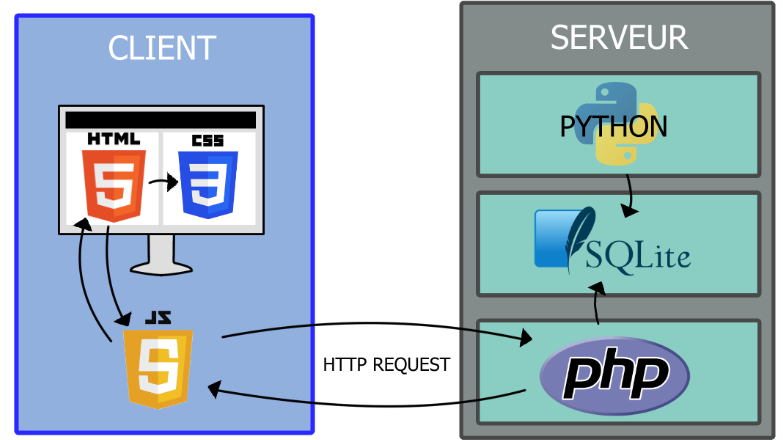
\includegraphics[scale=0.45]{./img_rapport/shema_global.png}
    \caption{Résumé du fonctionnement global du site}
    \label{fig-page-web-v1}
  \end{figure}

\end{document}
